\documentclass[12pt]{article} 
\usepackage{longtable}
\usepackage{makecell}
\usepackage{float}
\usepackage{graphicx}
\usepackage{bm}
\usepackage{placeins}
\usepackage{booktabs}
\usepackage{gensymb}
\usepackage{amssymb}
\usepackage{indentfirst}
\usepackage{threeparttable} 
\usepackage{multirow}
\usepackage{subfigure} % 导言区引入
\usepackage{tabularx}
\usepackage{aligned-overset}
\usepackage[slantfont,boldfont]{xeCJK}
\usepackage{fontspec}
\renewcommand{\arraystretch}{1.5}
% \usepackage[paperwidth=21cm,paperheight=29.7cm]{geometry}
\usepackage[a4paper,margin=2cm]{geometry}
\setCJKmainfont{SimSun}
\setmainfont{SimSun}
\setsansfont{SimSun}
% 设置正文字体为四号（12pt）
% \renewcommand{\CJKmainfont}{SimSun}
\renewcommand{\CJKfamilydefault}{\CJKrmdefault}
\renewcommand{\normalsize}{\fontsize{12pt}{18pt}\selectfont}
\normalsize

\title{牛顿环实验报告}
\author{2411545 邱凯锐}
\date{2025.11.21}

\begin{document}
\maketitle
\section{实验目的}
1. 观察等厚干涉现象，并利用等厚干涉测量凸透镜表面的曲率半径 

2. 了解读数显微镜的使用方法

\section{实验原理}
当曲率半径为 $R$ 的平凸透镜放置在一平板玻璃上时，在透镜和平板
玻璃之间形成一个厚度变化着的空气间隙，如 Figure 1 所示。当光线垂直照
射到其上，从空气间隙的上下表面反射的两束光线 ① 、 ② 将在空气间隙
的上表面附近实现干涉叠加，两束光之间
的光程差 $\Delta$ 随空气间隙的厚度变化而变
化，空气间隙厚度相同处的两束光具有相
同的光程差，所以干涉条纹是以接触点为
圆心的一组明暗相间的同心圆环，称为牛
顿环。中心干涉暗环的级次为 0 ，向外逐次
增加，亮环的级次从 1 开始，向外逐次增加，
离中心最近的亮环级次为 1。牛顿环是一个
典型的分振幅等厚干涉。

\begin{figure}[H]
    \centering
    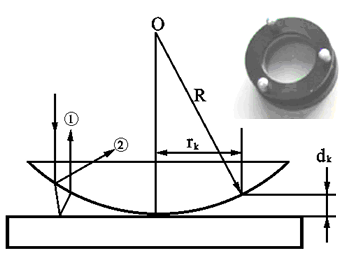
\includegraphics[width=0.5\textwidth]{fig 1.png}
    \caption{牛顿环装置}
\end{figure}

在 Figure 1 中，$R$ 为被测透镜凸面的曲率半径，
$r_k$ 是第 $k$ 级干涉环的半
径， 
$d+k$ 是第 $k$ 级干涉环所对应的空气间隙的厚度。如果入射光的波长为
 $\lambda $
，则第 $k$ 级干涉环所对应的光程差为：
\begin{equation}
    \Delta_k=2d_k+\lambda/2
\end{equation} 

其中，$\lambda/2$ 为光由光疏介质入射到光密介质时，反射光的半波损失。因此，在接触点处 $d_k=0$ 的光程差为：
\begin{equation}
    \Delta_0=\lambda/2
\end{equation}

在理想情况下，牛顿环的中心是一个几何暗点。但在实际情况中，
透镜和平板玻璃接触时，由于有重力和压力存在，透镜的凸面和平板玻
璃均发生形变，两者的接触不再是点接触，而是面接触。因此，牛顿环
的零级暗条纹不是个点，而是一个较大的暗斑。 

第 $k$ 级干涉暗环处的光程差为
\begin{equation}
    \Delta_k=2d_k+\lambda/2=(k+1/2)\lambda
\end{equation}
所对应的空气间隙的厚度为
\begin{equation}
    d_k=k\lambda/2
\end{equation}
在 Figure 1 中，因 $R>>d_k$ ，所以有
\begin{equation}
    r_k^2=R^2-(R-d_k)^2\approx 2Rd_k
\end{equation}
由式（4）和（5）可知，第 $k$ 级干涉暗环的半径为
\begin{equation}
    r_k=\sqrt{k\lambda R}
\end{equation}

\begin{figure}[H]
    \centering
    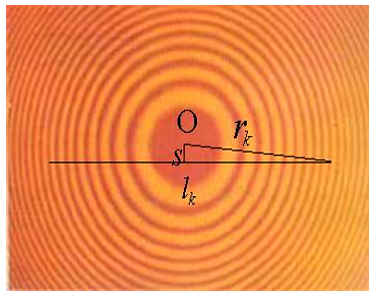
\includegraphics[width=0.5\textwidth]{fig 2.png}
    \caption{干涉环的测量}
\end{figure}

在实际测量中，由于无法准确确定
干涉环的圆心所在位置，这样就不可能准
确地测量干涉环的半径。因此，直接利用
式（6）作为测量公式将对测量结果带来
很大的误差。事实上，在测量中可以准确
地获得各个级次干涉环的弦长。假设这个
弦到圆心的距离是 $s$ ，由 Figure 2 中的几何关系可知： 
\begin{equation}
    l_k^2=4\left(r_k^2-s^2 \right)
\end{equation}

将式（6）代入式（7），可以得到所测弦长与透镜曲率半径之间满足以下关系
\begin{equation}
    l_k^2=4k\lambda R-4s^2
\end{equation}

根据式（8）对测量数据进行拟合得到直线斜率 $4\lambda R$ ，即可求得凸透镜的曲率半径 $R$

\section{实验仪器}
\begin{itemize}
    \item 牛顿环装置
    \item 钠灯
    \item 读数显微镜：测量过程中单向测量，避免回空差带来的实验误差
\end{itemize}

\begin{figure}[H]
    \centering
    \begin{minipage}{0.25\textwidth}
        \centering
        
\includegraphics[width=\textwidth]{fig1.jpg}
        \caption{牛顿环}
    \end{minipage}
    \begin{minipage}{0.25\textwidth}
        \centering
        
\includegraphics[width=\textwidth]{fig3.jpg}
        \caption{钠灯}
    \end{minipage}
    \begin{minipage}{0.25\textwidth}
        \centering
        
\includegraphics[width=\textwidth]{fig2.jpg}
        \caption{读数显微镜}
    \end{minipage}
\end{figure}

\section{实验内容}
1. 按 Figure 6 安排实验装置

2. 点燃钠灯，几分钟后它将发出明亮的黄光。调节半透半反镜的倾角
和左右方向，使显微镜的视场达到最亮。

3.调节显微镜的物镜，使自己能清
楚地看到叉丝。对显微镜进行调
焦，找到干涉条纹，并尽量使叉
丝与干涉环的中心重合。

4.测量不同级次干涉环的弦长。测
量时应测量较高级次的干涉环，
这样可以避免中心部分有形变带
来的测量误差。

\begin{figure}[H]
    \centering
    \begin{minipage}{0.3\textwidth}
        \centering
        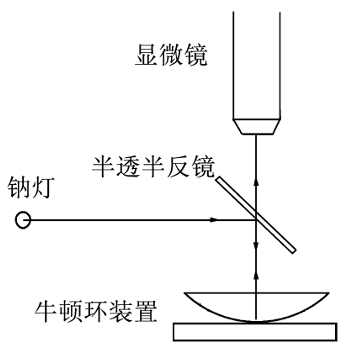
\includegraphics[width=\textwidth]{fig 3.png}
        \caption{实验装置示意图}
    \end{minipage}
    \hfil
    \begin{minipage}{0.3\textwidth}
        \centering
        
\includegraphics[width=\textwidth]{fig4.jpg}
        \caption{干涉环}
    \end{minipage}
\end{figure}


\section{实验数据}

\begin{table}[H]
\centering
\caption{牛顿环实验数据}
\vspace{1em}
\small
\setlength{\tabcolsep}{10pt}    % 调小列间距
\renewcommand{\arraystretch}{1.35}
\begin{tabular}{c*{7}{c}}
\hline\hline
级次 $k$ & 10 & 15 & 20 & 25 & 30 & 35 & 40 \\
左边位置 & 31.454 & 32.034 & 32.539 & 32.993 & 33.420 & 33.729 & 34.056 \\
右边位置 & 24.788 & 24.162 & 23.618 & 23.151 & 22.740 & 22.326 & 21.951 \\
弦长 $l_k$ (mm) & 6.666 & 7.872 & 8.921 & 9.842 & 10.680 & 11.403 & 12.105 \\
弦长平方 $l_k^2$ & 44.436 & 61.968 & 79.584 & 96.865 & 114.062 & 130.028 & 146.531 \\
\hline\hline
\end{tabular}
\end{table}

\begin{figure}[H]
    \centering
    
\includegraphics[width=0.7\textwidth]{Figure_1.png}
\end{figure}

对实验数据进行曲线拟合，得
\begin{equation}
    l^2= 3.406319 k +11.052744
\end{equation}
决定系数为
\begin{equation}
    R^2=0.9997
\end{equation}
计算得到凸透镜的曲率半径为
\begin{equation}
    R=1.45\ \mathrm{m}
\end{equation}

\section{思考题}

1. \textbf{为什么不能利用式（6）作为测量公式？}

在实际测量中，由于无法准确确定
干涉环的圆心所在位置，这样就不可能准
确地测量干涉环的半径。因此，直接利用
式（6）作为测量公式将对测量结果带来
很大的误差。

2. \textbf{如果实验中采用鼓轮读数装置的读数显微镜，测量中如何避免回空
差？}

始终保持单向测量。

3. \textbf{为了获得被测透镜的曲率半径，为什么不能对低级次的干涉环进行
测量？}

避免中心部分有形变带
来的测量误差。

4. \textbf{为什么在调节半透半反镜时，要求显微镜的视场达到最亮？}

显微镜视场亮度与进入它的总光功率直接相关。
当你调节半透镜角度和位置时，你实际上在改变两束光（来自两臂）在显微镜物平面上的重合程度。视场越亮表示：

（1）两束光的光斑重合最完全

（2）进入显微镜光阑的光量最大

（3）意味着分束器角度正确、光路对准良好

5. \textbf{在实验装置调整完毕后，怎样才能在最短的时间内完成所要求的测
量任务？}

采取单向测量的方法，从高级次到低级次再到高级次进行测量。

6. \textbf{估计白光下不同颜色和级次的干涉环所对应的空气间隙的厚度。}

\begin{table}[H]
\centering
\caption{不同颜色与级次对应的空气间隙厚度（暗纹 $\Delta=\frac{m\lambda}{2}$）}
\renewcommand{\arraystretch}{1.2}
\begin{tabular}{cccccc}
\toprule
级次 $m$ 
& 红（650 nm） 
& 黄（589 nm） 
& 绿（546 nm） 
& 蓝（486 nm） 
& 紫（436 nm） \\
\midrule
0 & 0 nm  & 0 nm & 0 nm & 0 nm & 0 nm \\
1 & 325 nm  & 294.5 nm & 273 nm  & 243 nm & 218 nm \\
2 & 650 nm  & 589 nm  & 546 nm & 486 nm  & 436 nm  \\
3 & 975 nm  & 883.5 nm & 819 nm  & 729 nm  & 654 nm  \\
4 & 1300 nm  & 1178 nm  & 1092 nm  & 972 nm  & 872 nm  \\
5 & 1625 nm  & 1472.5 nm  & 1365 nm  & 1215 nm  & 1090 nm  \\
\bottomrule
\end{tabular}
\end{table}

7. \textbf{是否可以利用亮环进行本实验中的测量，如果可以，导出测量公式。
并说明测量方法。}

第 $k$ 级干涉亮环处的光程差为
\begin{equation}
    \Delta_k=2d_k+\lambda/2=k\lambda
\end{equation}
对应的空气间隙厚度为
\begin{equation}
    d_k=(2k-1)\lambda/4
\end{equation}
对应的干涉亮环的半径为
\begin{equation}
    r_k=\sqrt{\frac{(2k-1)\lambda R}{2}}
\end{equation} 
和式（7）同理写出
\begin{equation}
    l_k^2=4(r_k^2-s^2)=4k\lambda R-2\lambda R -4s^2
\end{equation}
测量方法和暗环的一致。

8. \textbf{如果实验中，将牛顿环装置中的平板玻璃换成一个表面为凹球面的
玻璃，并且凹面的曲率半径大于等于待测凸透镜的表面曲率半径。
在这种情况下，如何测量待测透镜的曲率半径？这种测量方法实际
上是光学加工中检查透镜质量所采用的方法，带凹面的玻璃被称为
模板。}

设模板的曲率半径为 $R_0$。
由式（4），空气膜厚度为 $d_k=k\lambda/2$ 。根据几何关系，有
\begin{equation}
    \sqrt{R_0^2-r_k^2}-\sqrt{R^2-r_k^2}=d_k+R_0-R
\end{equation}
由于 $r_k<<R<R_0$，忽略小量，有
\begin{equation}
    r_k^2=2d\frac{R_0R}{R_0+R}=\frac{R_0R\lambda}{R_0+R}k
\end{equation} 
对应的弦长为
\begin{equation}
    l_k^2=4(r_k^2-s^2)=\frac{4R_0R\lambda}{R_0+R}k-4s^2
\end{equation}
测量方法和平板玻璃片一致，拟合曲线得到斜率即可计算出待测透镜的曲率半径 $R$ 。


\end{document}